\begin{figure}[ht]\label{fig:cell}
\begin{center}



\tikzset{every picture/.style={line width=0.75pt}} %set default line width to 0.75pt        

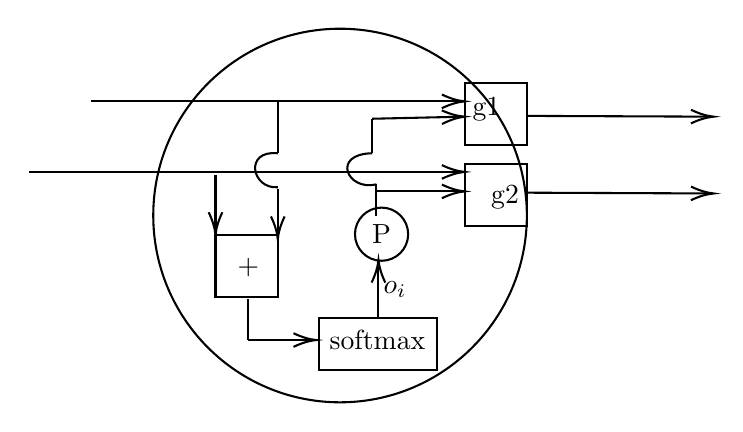
\begin{tikzpicture}[x=0.75pt,y=0.75pt,yscale=-1,xscale=1]
%uncomment if require: \path (0,247.3125); %set diagram left start at 0, and has height of 247.3125

%Shape: Circle [id:dp6083722186206264] 
\draw   (300,90) .. controls (300,40.29) and (340.29,0) .. (390,0) .. controls (439.71,0) and (480,40.29) .. (480,90) .. controls (480,139.71) and (439.71,180) .. (390,180) .. controls (340.29,180) and (300,139.71) .. (300,90) -- cycle ;
%Straight Lines [id:da561245922461306] 
\draw    (270,35) -- (448,35) ;
\draw [shift={(450,35)}, rotate = 180] [color={rgb, 255:red, 0; green, 0; blue, 0 }  ][line width=0.75]    (10.93,-3.29) .. controls (6.95,-1.4) and (3.31,-0.3) .. (0,0) .. controls (3.31,0.3) and (6.95,1.4) .. (10.93,3.29)   ;

%Straight Lines [id:da18790606634377727] 
\draw    (240,69) -- (448,69) ;
\draw [shift={(450,69)}, rotate = 180] [color={rgb, 255:red, 0; green, 0; blue, 0 }  ][line width=0.75]    (10.93,-3.29) .. controls (6.95,-1.4) and (3.31,-0.3) .. (0,0) .. controls (3.31,0.3) and (6.95,1.4) .. (10.93,3.29)   ;

%Shape: Square [id:dp2745914981980191] 
\draw   (450,26) -- (480,26) -- (480,56) -- (450,56) -- cycle ;
%Shape: Square [id:dp4400376186234609] 
\draw   (450,65) -- (480,65) -- (480,95) -- (450,95) -- cycle ;
%Shape: Square [id:dp5494449586600998] 
\draw   (330,99.38) -- (360,99.38) -- (360,129.38) -- (330,129.38) -- cycle ;
%Straight Lines [id:da5818908117859822] 
\draw    (345.5,150) -- (376.5,150) ;
\draw [shift={(378.5,150)}, rotate = 180] [color={rgb, 255:red, 0; green, 0; blue, 0 }  ][line width=0.75]    (10.93,-3.29) .. controls (6.95,-1.4) and (3.31,-0.3) .. (0,0) .. controls (3.31,0.3) and (6.95,1.4) .. (10.93,3.29)   ;

%Shape: Rectangle [id:dp8507803775022897] 
\draw   (380,139.38) -- (436.5,139.38) -- (436.5,164.38) -- (380,164.38) -- cycle ;
%Straight Lines [id:da5079909504409219] 
\draw    (408.5,139.38) -- (408.5,113.38) ;
\draw [shift={(408.5,111.38)}, rotate = 450] [color={rgb, 255:red, 0; green, 0; blue, 0 }  ][line width=0.75]    (10.93,-3.29) .. controls (6.95,-1.4) and (3.31,-0.3) .. (0,0) .. controls (3.31,0.3) and (6.95,1.4) .. (10.93,3.29)   ;

%Straight Lines [id:da24915260067311573] 
\draw    (330,70.38) -- (330,97.38) ;
\draw [shift={(330,99.38)}, rotate = 270] [color={rgb, 255:red, 0; green, 0; blue, 0 }  ][line width=0.75]    (10.93,-3.29) .. controls (6.95,-1.4) and (3.31,-0.3) .. (0,0) .. controls (3.31,0.3) and (6.95,1.4) .. (10.93,3.29)   ;

%Straight Lines [id:da08640126621337885] 
\draw    (360,35) -- (360,60) ;


%Straight Lines [id:da7146155948789545] 
\draw    (360,77.38) -- (360,99.38) ;
\draw [shift={(360,101.38)}, rotate = 270] [color={rgb, 255:red, 0; green, 0; blue, 0 }  ][line width=0.75]    (10.93,-3.29) .. controls (6.95,-1.4) and (3.31,-0.3) .. (0,0) .. controls (3.31,0.3) and (6.95,1.4) .. (10.93,3.29)   ;

%Curve Lines [id:da3867366642345542] 
\draw    (360,76.38) .. controls (347.5,77.38) and (343.5,58.38) .. (360,60) ;


%Straight Lines [id:da5452257068640174] 
\draw    (345.5,130.38) -- (345.5,150) ;


%Straight Lines [id:da40110507885008895] 
\draw    (407.5,75) -- (407.5,90) ;


%Curve Lines [id:da38530851203182825] 
\draw    (407.5,75) .. controls (393.5,78.38) and (385.5,60.38) .. (405.5,60) ;


%Straight Lines [id:da4735381882476042] 
\draw    (405.5,43.38) -- (448,42.42) ;
\draw [shift={(450,42.38)}, rotate = 538.71] [color={rgb, 255:red, 0; green, 0; blue, 0 }  ][line width=0.75]    (10.93,-3.29) .. controls (6.95,-1.4) and (3.31,-0.3) .. (0,0) .. controls (3.31,0.3) and (6.95,1.4) .. (10.93,3.29)   ;

%Straight Lines [id:da9357133547762917] 
\draw    (405.5,43.38) -- (405.5,60) ;


%Straight Lines [id:da9994096101128709] 
\draw    (407.5,78.38) -- (448,78.38) ;
\draw [shift={(450,78.38)}, rotate = 180] [color={rgb, 255:red, 0; green, 0; blue, 0 }  ][line width=0.75]    (10.93,-3.29) .. controls (6.95,-1.4) and (3.31,-0.3) .. (0,0) .. controls (3.31,0.3) and (6.95,1.4) .. (10.93,3.29)   ;

%Straight Lines [id:da6130989952789851] 
\draw    (480,42) -- (568,42.37) ;
\draw [shift={(570,42.38)}, rotate = 180.24] [color={rgb, 255:red, 0; green, 0; blue, 0 }  ][line width=0.75]    (10.93,-3.29) .. controls (6.95,-1.4) and (3.31,-0.3) .. (0,0) .. controls (3.31,0.3) and (6.95,1.4) .. (10.93,3.29)   ;

%Straight Lines [id:da28139602174802314] 
\draw    (480,79) -- (568,79.37) ;
\draw [shift={(570,79.38)}, rotate = 180.24] [color={rgb, 255:red, 0; green, 0; blue, 0 }  ][line width=0.75]    (10.93,-3.29) .. controls (6.95,-1.4) and (3.31,-0.3) .. (0,0) .. controls (3.31,0.3) and (6.95,1.4) .. (10.93,3.29)   ;


% Text Node
\draw (345.81,115.19) node  [align=left] {+};
% Text Node
\draw (408,150) node  [align=left] {softmax};
% Text Node
\draw (416.5,125.5) node  [align=left] {$\displaystyle o_{i}$};
% Text Node
\draw    (410, 99) circle [x radius= 12.81, y radius= 12.81]   ;
\draw (410,99) node  [align=left] {P};
% Text Node
\draw (460.5,39) node  [align=left] {g1};
% Text Node
\draw (469.5,81) node  [align=left] {g2};


\end{tikzpicture}


\end{center}
\caption{Cell}
\end{figure}

